% Статья про разработку QReal:Robots и применение DSM-подхода, для сборника кафедры

\documentclass[a4paper]{article}
\usepackage[a4paper, top=17mm, bottom=17mm, left=17mm, right=17mm]{geometry}
\usepackage[utf8]{inputenc}
\usepackage[T2A,T1]{fontenc}
\usepackage[colorlinks,filecolor=blue,citecolor=green,unicode,pdftex]{hyperref}
\usepackage{cmap}
\usepackage[english,russian]{babel}
\usepackage{amsmath}
\usepackage{amssymb,amsfonts,textcomp}
\usepackage{color}
\usepackage{array}
\usepackage{hhline}
\hypersetup{colorlinks=true, linkcolor=blue, citecolor=blue, filecolor=blue, urlcolor=blue, pdftitle=1, pdfauthor=, pdfsubject=, pdfkeywords=}
\usepackage{graphicx}
\usepackage{indentfirst}
\usepackage{cite}
\usepackage{literat}
%\usepackage{wrapfig}

\sloppy
\pagestyle{plain}

\title{Применение DSM-платформы QREAL при разработке среды программирования роботов QReal:Robots}

\author{Ю.В.Литвинов \\ ст. преп. кафедры системного программирования СПбГУ, \\ инженер-программист ЗАО ``Ланит-Терком'' \\ yurii.litvinov@gmail.com}
\date{}
\begin{document}

\maketitle
\thispagestyle{empty}

\renewcommand{\thefootnote}{}
\footnote{\small{\copyright~Ю.В.Литвинов,~2012.}}
\renewcommand{\thefootnote}{\arabic{footnote}}
\setcounter{footnote}{0}

\begin{quote}
\small\noindent
В российских школах сейчас активно идёт внедрение робототехнических конструкторов Lego Mindstorms NXT для преподавания информатики. Для программирования таких роботов обычно используются визуальные языки, однако, сред разработки, полностью удовлетворяющих школьных учителей, сейчас не существует. Поэтому была произведена попытка применить DSM-платформу QReal для разработки такого средства. В статье описывается функциональность существующих средств программирования роботов, даётся краткий обзор архитектуры системы QReal, описывается созданный язык программирования роботов и роль средств метамоделирования QReal в процессе его создания. Делаются выводы о том, насколько эффективным оказался DSM-подход в решении поставленной задачи и какой ещё функциональностью должна обладать DSM-платформа, чтобы ещё повысить эффективность создания языка и инструментальных средств для него.
\end{quote}

\section*{Введение}
Сейчас в школах для преподавания информатики активно внедряются робототехнические конструкторы. Детям проще создавать свои первые программы, если они видят, как физический, осязаемый объект исполняет описанные в программе команды. Самым популярным на данный момент робототехническим набором является конструктор Lego Mindstorms NXT~\cite{legoNxt}. Он позволяет из блока управления, моторов и нескольких видов датчиков (датчики касания, расстояния, света и другие) собирать несложные устройства, которые могут исполнять команды с компьютера по интерфейсу Bluetooth или исполнять программу, загруженную в блок управления.

Для программирования этого конструктора существует несколько как текстовых, так и визуальных сред программирования. На первых этапах обучения обычно используют визуальные среды, такие как NXT-G или Robolab~\cite{robolabHome}. Однако существующие популярные среды обладают рядом недостатков, делающих их использование затруднительным --- отсутствие полного перевода на русский язык, высокая стоимость, неудобный пользовательский интерфейс, недостаточная функциональность. Таким образом, существует потребность в разработке системы визуального программирования для Lego Mindstorms NXT, специально предназначенной для применения в российских школах.

Это делает область визуального программирования роботов весьма привлекательной для апробации средств предметно-ориентированного визуального программирования. На кафедре системного программирования Санкт-Петербургского Государственного Университета уже несколько десятилетий занимаются исследованиями в области визуальных языков и их применением в области раработки систем реального времени и встроенных систем~\cite{videoDsl}\cite{dsmPlatforms}\cite{real1}\cite{real2}\cite{student1}\cite{student2}. В частности, с 2007 года существует и активно развивается проект QReal~\cite{qReal}. В рамках этого проекта исследуются средства создания визуальных предметно-ориентированных языков, называемые также domain-specific modelling-, или DSM-средства. Поскольку визуальный язык программирования роботов является хорошим примером предметно-ориентированного языка, было решено применить имевшиеся результаты для разработки системы программирования роботов. 

В статье описано, с какими трудностями пришлось столкнуться в ходе разработки, чем помог DSM-инструментарий, чем он не смог помочь, и делаются выводы о том, какими функциями должна обладать система создания визуальных сред программирования, чтобы быть полезной для решения реальных задач. Изложенные в статье результаты могут быть интересны тем, что разрабатываемую с помощью DSM-инструментария CASE-систему удалось довести до состояния, в котором её смогли успешно использовать люди, занимающиеся робототехникой и далёкие от программирования, в том числе и ученики пятых-шестых классов. Таким образом, по результатам этой апробации DSM-подход доказал свою применимость не только как средство создания специализированных инструментов для узкого круга пользователей, но и для разработки сред, предназначенных для массового потребителя и используемых в образовательных и развлекательных целях. Разработанная нами среда QReal:Robots была представлена на ряде конференций и семинаров школьных учителей, роботы, запрограммированные с её помощью студентами, выступали на городских и всероссийских робототехнических фестивалях и соревнованиях. По отзывам конечных пользователей --- учеников школ --- среда QReal:Robots удобнее, чем используемые ими средства программирования, и обладает более дружественным пользовательским интерфейсом.

\section{Мотивация}
Идея использовать роботов при начальном обучении информатике родилась неслучайно. Проблема, на которую указывал ещё Ф.~Брукс в своей известной книге ``Мифический человеко-месяц''~\cite{mythicalManMonth}, заключается в том, что программы нематериальны, их невозможно увидеть. Кроме того, даже представить себе программу не так просто --- каждый человек ``видит'' программу по-разному. Людям, которые программируют впервые, приходится сразу же работать с абстрактными понятиями, и судить о правильности своих программ они могут только по внешним проявлениям их работы --- какой ответ программа выведет на экран. При этом может быть совсем не очевидно, как программа работает, и что делать, если выводимый ею ответ неправильный, что нужно делать, чтобы получить правильный ответ, к тому же часто случается так, что программа работает неправильно, но правильный ответ всё-таки выводит. Всё это делает изучение информатики весьма сложным.

И отечественные, и зарубежные методисты давно осознают эту проблему, поэтому традиционно начальное обучение информатике проводится с использованием концепции исполнителя --- некоторого, зачастую воображаемого, устройства, способного выполнять простые команды в некотором простом окружении. Один из самых известных исполнителей, применяемых в школах --- ``черепашка'' LOGO~\cite{logo}, разработанная американским программистом, психологом и педагогом Сеймуром Пейпертом в 1967 году. Исполнитель ``черепашка'' может перемещаться по экрану, оставляя за собой след, которым вычерчиваются различные фигуры. Черепашка подчиняется командам простого интерпретируемого языка, позволяющего описывать её перемещения и повороты. Таким образом, процесс исполнения программы визуализируется движением исполнителя по экрану, и если программа работает неправильно, это будет сразу видно. 

В Советском Союзе преподавание информатики как школьного предмета началось во многом благодаря усилиям академика А.П.~Ершова и его коллектива, в который входили Г.А.~Звенигородский и Н.А.~Юнерман. Ими была разработана отечественная учебная система ``Робик''~\cite{robik}, основанная в основном на тех же принципах, что и LOGO. Ими же были разработаны методики и программы преподавания информатики в школах, где понятие ``исполнитель'' занимало ключевую позицию.

Однако исполнитель, перемещающийся по экрану, всё же недостаточно нагляден. Сеймур Пейперт в своих экспериментах использовал механическую черепашку~\cite{logoTurtle} --- реальный, осязаемый объект, исполняющий программу, что оказалось гораздо понятнее для школьников, чем черепашка, движущаяся по экрану. Современные технологии позволяют создавать недорогие механические устройства, управляемые загружаемой в них программой, либо непосредственно с компьютера, поэтому идея использования материальных исполнителей в школьной информатике получила второе рождение, из-за чего получил распространение конструктор Lego Mindstorms NXT. Для преподавания информатики с использованием этого конструктора существуют методические пособия (например,~\cite{filippov}). 

Однако, робототехнический конструктор довольно сложно программировать: из набора деталей могут быть собраны самые разные конструкции, поэтому программировать приходится в терминах оборотов моторов, подключённых к определённым портам управляющего блока, а не в терминах движений и поворотов. Это, безусловно, делает процесс обучения более творческим, поскольку школьники могут собрать своего собственного исполнителя, но и более сложным с точки зрения написания для этого исполнителя программ. Проблема сложности программирования преодолевается использованием наглядных визуальных языков и удобных графических редакторов для составления программ из блоков, представляющих элементарные команды, такие как ``включить мотор'', ``гудок'' и т.д. Таким образом, начинающие работают с графическими языками программирования, а более опытные школьники постепено переходят на текстовые C-образные языки. В комплекте с конструктором поставляется графическая среда программирования NXT-G, поэтому визуальные языки среди использующих Mindstorms NXT весьма популярны.

В проекте QReal~\cite{qReal} ведутся исследования в области визуальных языков, в частности, в области предметно-ориентированного визуального программирования. Предметно-ориентированный подход к созданию программного обеспечения основан на том, что иногда задачу проще решать, создав для её решения специализированный язык, чем использовать язык общего назначения. Разумеется, создавать визуальный язык и средства его поддержки (такие как редактор диаграмм, генераторы кода) ``с нуля'' было бы слишком трудозатратно и свело бы на нет все преимущества от узкой специализированности языка. Поэтому создаются средства, позволяющие автоматизировать часть этого процесса. Если обычные среды для визуального моделирования и визуального программирования называют CASE-средствами, то средства для создания таких сред называют обычно metaCASE-средствами. QReal --- пример metaCASE-системы.

Программирование роботов является интересной предметной областью для апробации metaCASE-системы. С одной стороны, использование визуальных языков программирования довольно широко распространено среди людей, занимающихся робототехникой, поэтому здесь можно рассчитывать на содержательное сравнение с существующими решениями и обратную связь от пользователей, уже знакомых с различными визуальными языками. С другой стороны, программирование роботов --- хороший пример предметной области, достаточно узкой, чтобы можно было получить заметное преимущество от создания для неё специализированного языка, и вместе с тем достаточно содержательной, чтобы такой специализированный язык был нетривиальным и мог бы послужить примером для исследования решений, применимых в других содержательных случаях. Типичные программы для роботов состоят из элементарных команд, таких как ``включить моторы'', ``ожидать такое-то показание сенсора'' и т.д., и управляющих конструкций, таких как условные операторы и циклы. На языке общего назначения такие команды были бы вызовами программного интерфейса (Application Programming Interface, далее --- API) операционной системы или библиотек робота и требовали бы для себя различных вспомогательных конструкций, таких как операторы включения и объявления переменных, а на специализированном языке каждая такая команда представляется одним блоком, для использования которого достаточно просто разместить его на диаграмме. Это существенно снижает требования к знаниям программиста и снижает вероятность ошибки в программе --- например, невозможно опечататься при указании имени вызываемой функции. Вместе с тем, многие языковые конструкции, типичные для императивного программирования, такие как ветвления и циклы, будут присутствовать и в этом языке, так что если удастся подобрать удобное графическое представление для программ для роботов, можно надеяться обобщить полученный результат на другие задачи, хорошо выражаемые в императивных терминах.

\section{Средства визуального программирования роботов}
Рассмотрим существующие средства визуального программирования роботов. Поскольку в контексте данной работы нас интересует использование роботов в школьной информатике, основной акцент в обзоре будет сделан на свойства продуктов, которые важны именно в этой сфере. Перечислим эти свойства.
\begin{itemize}
  \item Возможность создавать довольно сложные программы, включающие в себя нетривиальные математические выражения, циклы, ветвления, переменные, параллельные задачи --- применение таких средств должно дать возможность иллюстрировать содержательный материал из информатики и кибернетики, например, понятие регуляторов.
  \item Простота и удобство в работе. Неудобный пользовательский интерфейс создаёт дополнительную когнитивную нагрузку на школьников и усложняет восприятие и без того сложного материала.
  \item Наличие встроенных средств отладки, чтобы школьники могли следить за ходом выполнения своей программы и её состояниями, имели бы инструмент для эффективного поиска ошибок.
  \item Возможность перехода от графической формы программы к текстовой, чтобы школьники старших классов, серьёзно занимающиеся программированием, имели возможность смотреть, как их программа выглядит на более приближенном к индустриальному программированию текстовом языке, и могли бы, возможно, вносить в текстовую программу правки в той же среде, в которой они привыкли работать.
  \item Необходима русскоязычная среда разработки, поскольку школьники зачастую ещё не владеют иностранными языками, а необходимость работать со словарём существенно усложняет восприятие материала.
  \item Цена --- каким бы хорошим ни был продукт, если он стоит дорого, не все школы могут себе его позволить.
  \item Желательно, чтобы продукт продолжал развиваться и адаптироваться к новым операционным системам и аппаратному обеспечению.
\end{itemize}
Основные среды программирования, распространённые на данный момент, рассмотрены ниже с точки зрения перечисленных критериев.

\subsection{Среда NXT-G}
Среда NXT-G --- единственное средство программирования, которое поставляется в комплекте с конструктором Lego Mindstorms NXT. Среда базируется на системе LabView, среде визуального программирования от компании National Instruments. В LabView в качестве языка программирования используется визуальный язык G (из-за чего NXT-G и получила своё название). Язык G моделирует процесс вычислений, ориентированный на данные, в котором явно задаётся не последовательность выполнения операторов, а связи между блоками по данным. Блок программы может предоставлять некоторые выходные данные, которые могут служить входными данными для другого блока. Блоки начинают исполняться, когда имеют данные на всех входах. Если сразу несколько блоков имеют данные на всех входах, они исполняются параллельно. Такой подход довольно сильно отличается от подхода, принятого в императивном программировании, однако же довольно распространён среди инженеров и учёных. Например, на тех же принципах основана другая известная визуальная среда програмирования научных вычислений и моделирования Matlab/Simulink.

Основная проблема этой среды состоит в довольно слабой поддержке математических выражений. Математические формулы здесь, как и вся программа, строятся из блоков. Есть блоки арифметических операций, блоки чтения и записи значения в переменную, блок, считывающий значение константы, блоки, считывающие показания с сенсоров. Таким образом, даже чтобы запрограммировать несложную формулу, требуется изображать блоками дерево разбора выражения, которое эту формулу задаёт. Для иллюстрации серьёзности этой проблемы достаточно сказать, что программа, представляющая пропорционально-дифференциальный регулятор для движения робота вдоль линии или вокруг препятствия, на языке C занимает порядка десятка строк, тогда как на NXT-G не помещается на одном экране и весьма сложна для понимания. Таким образом, первому из предложенных критериев --- пригодности для иллюстрации содержательного материала информатики и кибернетики --- NXT-G не соответствует. В основном поэтому NXT-G и не получил широкого распространения в школах.

Что касается простоты и удобства в работе, среда NXT-G специально создавалась для начинающих и поэтому довольно эргономична. По мнению некоторых пользователей она даже слишком эргономична, поскольку не даёт произвольно размещать блоки на диаграмме, автоматически (и не всегда удачно) прокладывает соединительные линии между блоками и т.д. Для применения NXT-G в школьных классах оказалась важна ещё такая его особенность: большая часть свойств элементов не отображается на диаграмме, а доступна только через редактор свойств, что делает невозможным показ всей программы на проекторе. Никаких средств отладки NXT-G не имеет, текстовая форма программы не порождается, русификация существует, но неофициальная. К плюсам продукта следует отнести то, что он распространяется вместе с конструктором и доступен для скачивания с сайта производителя бесплатно. Кроме того, продукт до сих пор развивается и обновляется. Средствами LabView возможно добавление сторонних блоков, кроме того, сам NXT-G позволяет выделить набор блоков в подпрограмму и использовать её как новый блок.

\subsection{Среда Robolab}
Среда Robolab~\cite{robolab} так же, как и NXT-G, базируется на среде LabView. Robolab специально создавалась для школьного образования и c самого начала своего развития учитывала пожелания школьных учителей и специфику преподавания в школах. Пример специфичного для школ решения, реализованного в Robolab --- наличие нескольких уровней возможностей среды. На самом простом уровне доступны только некоторые возможности визуального языка, и программа строится заполнением пустых мест в шаблоне посредством выбора блоков из всплывающего меню. Это позволяет создавать только самые простые программы, имеющие стандартную структуру: команды управления моторами, за которыми следует блок, ожидающий наступления какого-либо события. Причём, этот уровень имеет четыре подуровня, и на первых трёх подуровнях программа может состоять только из одного такого "шага". Сделано всё это для того, чтобы дать возможность детям в начальной школе или даже детском саду пользоваться программой --- в столь раннем возрасте они вполне могут не уметь читать. На втором уровне (который тоже состоит из нескольких подуровней) пользователи могут рисовать уже настоящие диаграммы, размещая произвольным образом блоки из палитры и соединяя их линиями, определяющими поток управления. Разница между подуровнями заключается в количестве доступных в палитре блоков, первые подуровни имеют меньше блоков с меньшим количеством параметров. Разбиение на уровни и подуровни организовано так, чтобы дети могли осваивать среду программирования практически без помощи учителя, руководствуясь лишь интуицией. Отзывы учителей, приведённые в~\cite{robolab}, показывают, что этой цели удалось достигнуть.

Математические выражения Robolab поддерживает гораздо лучше, чем NXT-G, позволяя писать произвольные выражения в текстовом виде. В Robolab имеется возможность использовать в формулах тригонометрические функции, обращаться напрямую к значениям показаний сенсоров. Циклы в Robolab реализованы довольно необычно --- есть блок "метка" и блок "переход к метке", передача управления никак больше не визуализируется. Имеются условные операторы, возможность порождать параллельные процессы, блоки для управления этими процессами, а также средства работы с подпрограммами. На Robolab можно просто и довольно удобно реализовать даже довольно сложные программы, и Robolab вполне подходит для иллюстрации материала из кибернетики до младших курсов вузов.

По другим критериям Robolab показывает несколько худшие характеристики. Программа была создана в конце 90-х годов, с тех пор интерфейс практически не менялся, поэтому сейчас выглядит несовременно. Кроме того, он довольно неудобен. Специализированных средств отладки в Robolab нет, хотя есть возможность снимать показания с робота и отображать на экране компьютера данные. Текстовое представление программы Robolab порождать не может. Русификация присутствует, но лишь частично, некоторые элементы управления не переведены. Robolab небесплатен, одна лицензия по стоимости сравнима с робототехническим набором, что для школ довольно дорого. Развитие Robolab идёт в основном путём добавления новых блоков, сама среда давно не изменялась.

Несмотря на указанные недостатки, Robolab на данный момент является основной средой, используемой в школах для разработки программ для роботов. По отзывам учителей, у многих имеется желание от него отказаться и заменить на что-нибудь более современное, однако пока на рынке не существует продуктов, которые могли бы составить ему серьёзную конкуренцию.

\subsection{Среда Microsoft Robotics Developer Studio}
Среда Microsoft Robotics Developer Studio~\cite{mrds} --- разработка компании Microsoft, предназначенная для программирования сложных многопоточных приложений с реактивной моделью поведения, используемых для управления робототехническими системами. Необходимость создания таких приложений есть не только в робототехнике, поэтому Robotics Developer Studio используется и для создания приложений, к робототехнике не относящихся (например, социальная сеть MySpace использует MRDS как составную часть серверного ПО~\cite{mrdsAtMySpace}). Программы в Robotics Developer Studio рисуются в виде диаграмм на визуальном языке VPL (Visual Programming Language), представляющем собой по сути визуализатор связей между отдельными параллельно исполняемыми компонентами (или веб-сервисами), из которых состоит программа. Система состоит из следующих крупных частей.

\begin{description}
  \item[Concurrency and Coordination Runtime (CCR)] --- библиотека для работы с параллельными и асинхронными потоками данных. Библиотека автоматизирует синхронизацию процессов, основываясь на потоках данных, так что прикладному программисту не надо задумываться об использовании семафоров, мониторов и прочих примитивов синхронизации. Библиотека позволяет прозрачно организовывать распределённые и параллельные вычисления, исполняя задачи на разных вычислительных устройствах. Это весьма полезно при программировании роботов, поскольку программы для роботов по природе реактивны и требуют обработки потоков данных одновременно с нескольких сенсоров, причём часть вычислений может быть сделана прямо на роботе, часть --- на компьютере вне него.
  \item[Decentralized Software Services (DSS)] --- среда времени выполнения, обеспечивающая представление компонентов программы в виде веб-сервисов и упрощающая организацию взаимодействия между ними. Взаимодействие между веб-сервисами ведётся по специальному протоколу Decentralized Software Services Protocol (DSSP). Инструменты, входящие в DSS, позволяют довольно легко конфигурировать веб-сервисы и связи между ними. DSS позволяет создавать распределённые приложения, которым не важно, на каком вычислительном устройстве выполняется тот или иной компонент, на одном из компьютеров робота или на компьютере вовне, лишь бы они были связаны единой сетью.
  \item[Visual Programming Language (VPL)] --- визуальный язык и редактор для него, используемый для конфигурирования сервисов. Сервисы можно перетащить на диаграмму, связать их входы и выходы, настроить их атрибуты. Получающаяся на таком языке диаграмма сильно напоминает диаграммы LabView, отображая зависимость между компонентами по данным.
  \item[Visual Simulation Environment (VSE)] --- трёхмерная среда симуляции поведения робота в виртуальном мире. Обладает довольно богатыми возможностями по симуляции физики и богатыми средствами отображения трёхмерной графики, что позволяет строить сложные и красиво выглядящие модели мира, с которым робот может взаимодействовать. В поставку среды включено несколько моделей окружения, в том числе модель квартиры, в которой работает так называемая "стандартная модель" робота, трёхколёсная платформа с установленным на ней ноутбуком, сенсором Microsoft Kinect\textregistered, инфракрасными датчиками расстояния и сонаром.
\end{description}

В школьном образовании, однако же, Microsoft Robotics Developer Studio используется очень редко. Причин этому несколько, главная из которых --- среда рассчитана в основном на симуляцию и не может эффективно взаимодействовать с реальным роботом. Для LEGO Mindstorms NXT есть возможность управления по каналу Bluetooth, но залить программу на робот возможности нет --- на роботе нет возможности запустить .NET-машину и нет ресурсов, необходимых для работы распределённых веб-сервисов. Реальные роботы, управляемые MRDS, обычно гораздо сложнее и дороже того, что можно использовать в школах (стандартная платформа, например, имеет в своём составе ноутбук, который один, скорее всего, дороже всего набора Mindstorms, хотя позиционируется как бюджетный робот, доступный каждому). Управления по Bluetooth недостаточно для решения задач, требующих малого времени реакции робота, из-за больших задержек посылки-приёма Bluetooth-пакетов, что делает MRDS неприменимой для большой области решаемых в школе задач. Симуляции же тоже оказывается недостаточно, потому что даже с хорошим физическим движком MRDS создаёт модель некоторого идеального мира, в котором большого количества проблем, решаемых алгоритмами кибернетики, просто не возникает. Даже простая задача, решаемая на реальном роботе, может оказаться нагляднее и полезнее школьникам, чем сложная программа, исполняемая на модели в симуляторе. А поскольку возможности быстро перейти от симулятора к реальному роботу нет, MRDS скорее занимает нишу "черепашки" Logo, применяясь в основном в виде исполнителя на экране.

Вторая важная причина очень узкого распространения MRDS в школах --- модель вычислений, в ней используемая. Представление программы в виде набора взаимосвязанных распределённых веб-сервисов может быть удобным для опытных программистов, но начинающим тяжело понять принципы, лежащие в основе такой модели программирования. Сложные механизмы взаимодействия веб-сервисов во многом спрятаны с помощью визуального языка VPL, но всё же требуется некоторое понимание происходящих в системе процессов для того, чтобы рисовать содержательные диаграммы. К тому же, блоки имеют довольно большое количество параметров, при задании которых используются различные сложные алгоритмические понятия, незнакомые начинающим программистам. В целом можно сказать, что MRDS больше подходит для студентов или профессиональных программистов, чем для школьников. Среда хоть и позволяет писать сколь угодно сложные программы, но делать это можно довольно нетривиальным и специфическим образом, что сильно снижает её ценность как иллюстративного материала.

Что касается других критериев, система довольно удобна в работе, имеет средства отладки и кодогенерации, однако, в силу своей специфики, эти средства довольно сложны для использования школьниками. Русификация системы отсутствует, однако же, система распространяется свободно и активно развивается.

\subsection{Выводы}
Сводная таблица с результатами сравнения существующих визуальных средств программирования роботов представлена ниже.

\begin{table}[h]
  \centering
    \begin{tabular} {| p{0.15\textwidth} | p{0.26\textwidth} | p{0.26\textwidth} | p{0.26\textwidth} |}
      \hline
                                            & NXT-G                                             & Robolab                                    & MRDS \\
      \hline
      Возможность создания сложных программ & Слабая поддержка сложных математических выражений & Присутствует всё, что требуется школьникам & Сколь угодно сложные программы \\
      \hline
      Простота и удобство в работе          & Довольно эргономично, но неудобно для уроков      & Устаревший интерфейс                       & Довольно удобна, но сложна \\
      \hline
      Средства отладки                      & Нет                                               & Нет                                        & Есть отладчик \\
      \hline
      Текстовое представление программы     & Нет                                               & Нет                                        & Генерирует код на C\# \\
      \hline
      Русификация                           & Неофициальная                                     & Частичная                                  & Нет \\
      \hline
      Цена                                  & Бесплатна                                         & Небесплатна                                & Бесплатна \\
      \hline
      Развитие                              & Развивается                                       & Расширение новыми блоками                  & Развивается \\
      \hline
    \end{tabular}
  \caption{Существующие среды}
  \label{tab:existingTools}
\end{table}

Можно сделать вывод, что существующие среды, кроме Robolab, слабо подходят для преподавания информатики и кибернетики в школах. Кроме того, как видно из таблицы, среда Robolab также имеет ряд существенных недостатков, наиболее важный из которых для школ --- высокая стоимость. Таким образом, существует потребность в создании бесплатной среды программирования, схожей по функциональности с Robolab, но имеющей средства отладки, генерации кода, русификацию и при этом удобную в работе.

\section{Предметно-ориентированное моделирование и система QReal}
Предметно-ориентированное визуальное моделирование --- весьма перспективная и развивающаяся в данный момент методология разработки программного обеспечения. Суть её состоит в том, что задача решается не с помощью языка общего назначения, такого как C++, Java, C\#, UML, а с помощью узкоспециализированного визуального языка, специально созданного для решения задач в данной предметной области или даже конкретно для решения поставленной задачи. Узкая направленность языка позволяет эффективно создавать на нём законченные программы, не требующие модификаций с использованием текстовых языков программирования. То, что специализированный язык близок к предметной области, позволяет использовать его даже людям, не владеющим программированием. Таким образом, для создания предметно-ориентированной технологии требуется небольшое количество высококвалифицированных программистов и аналитиков, после чего технологией может пользоваться большое количество низкоквалифицированных программистов либо непосредственно экспертов предметной области, что обходится дешевле, чем разработка системы традиционными средствами. Существуют хорошо известные текстовые предметно-ориентированные языки, такие как SQL, AWK, языки описания грамматик в конструкторах компиляторов. Исследования~\cite{kelly, kieburtz, weiss} показывают рост производительности труда программиста в 3-10 раз при использовании предметно-ориентированных языков по сравнению с программированием на текстовых языках общего назначения.

Разумеется, создавать специальный визуальный язык и разрабатывать для него индустриальные средства вручную было бы неразумно. Создание хорошей CASE-системы с нуля под силу только компаниям, которые на этом специализируются, и оправдано только в том случае, если эта CASE-система будет продаваться как коробочный продукт для массового покупателя, что противоречит самой идее предметно-ориентированного моделирования. Поэтому разрабатываются специальные инструментарии для быстрого создания визуальных языков и средств инструментальной поддержки для них, так называемые DSM-платформы. Любая такая платформа позволяет в том или ином виде описать синтаксис визуального языка и автоматически (или полуавтоматически) создать для него визуальный редактор. Некоторые DSM-платформы также позволяют задать для визуального языка правила генерации в текстовый целевой язык, описать набор доступных для языка инструментов и т.д. Наиболее зрелые на данный момент DSM-платформы --- Eclipse Graphical Modelling Project (GMP)~\cite{gmp}, MetaEdit+~\cite{metaEditPlus}, Visual Studio Visualization and Modeling SDK~\cite{vsvmsdk}, Microsoft Visio~\cite{visio}. 

Платформа Graphical Modelling Project базируется на среде Eclipse, а точнее, на двух библиотеках из состава Eclipse --- Eclipse Modeling Framework (библиотеке для работы с моделями) и Graphical Editing Framework (библиотеки для редакторов графов). Платформа довольно мощная, позволяет создавать отчуждаемые визуальные редакторы и генераторы кода, задавая метамодель языка в том числе с помощью стандарта обмена метамоделями XMI~\cite{xmi}, имеет открытый исходный код и распространяется свободно, являясь фактическим стандартом для осуществления научных исследований в области визуального моделирования и метамоделирования. Однако платформа довольно сложна для освоения и требует большого количества действий, чтобы получить редактор даже простого визуального языка. 

DSM-платформа MetaEdit+ --- наиболее зрелая на данный момент и активно используется в промышленном программировании. Имеет свой метаязык и графический метаредактор для описания абстрактного синтаксиса визуального языка, редактор формы элементов для задания конкретного синтаксиса, текстовый язык описания правил генерации целевого кода. Позволяет создавать отдельно работающие редакторы. Её основными недостатками являются её цена и то, что исходные коды этой системы закрыты.

Visual Studio Visualization and Modeling SDK (бывший Microsoft DSL Tools) позволяет создавать визуальные редакторы, встраиваемые в среду Microsoft Visual Studio 2010. На нём довольно удобно описывать простые визуальные языки, однако если требуется что-либо нестандартное (например, нестандарные фигуры элементов), требуется ручное кодирование на языке C\#. Распространяется бесплатно, но может применяться только в составе среды Visual Studio, стоимость которой довольно велика.

Среда Microsoft Visio позиционируется разработчиками скорее как векторный графический редактор, чем как DSM-платформа, однако содержит средства описания новых фигур, что даёт возможность использовать её в качестве легковесной DSM-платформы. Использование её в таком качестве оказалось удобным в том числе и в коммерческих проектах~\cite{videoDsl}. Однако же, Visio не обладает всей необходимой для DSM-платформы функциональностью --- нет полноценных средств описания метамодели, недостаточно функциональный программный интерфейс, затрудняющий работу с диаграммами сторонних инструментов, сложности с созданием нетривиальных фигур. Кроме того, среда небесплатная.

Помимо зрелых и известных DSM-платформ существует и некоторое количество академических разработок. Одна из таких разработок --- платформа QReal~\cite{qReal}, разрабатываемая на кафедре системного программирования Санкт-Петербургского Государственного Университета. QReal --- метаCASE-система, разрабатываемая как проект с открытым исходным кодом~\cite{qRealGithub}. На данный момент система QReal как DSM-платформа обладает следующими возможностями.
\begin{itemize}
  \item Задание метамодели разрабатываемого языка в текстовой форме в виде описания метамодели в специальном XML-формате либо в графической, с использованием метаредактора. Метаредактор в QReal сам реализован как предметно-ориентированный язык, существует его метамодель в виде XML-описания и для него применимы все возможности QReal, применимые к другим визуальным языкам.
  \item Задание формы фигур визуального языка с помощью встроенного графического редактора форм, представляющего собой по сути простой векторный графический редактор с поддержкой специфики языка, такой как возможность отображать значения логических свойств элемента прямо на фигуре. В качестве альтернативы есть возможность задавать форму фигуры непосредственно в XML-файле с описанием метамодели, в графическом формате, похожем на стандарт векторной графики SVG.
  \item Средства автоматической генерации кода редактора по метамодели и описаниям форм фигур. Редактор генерируется как код подключаемого модуля на языке C++ и подгружается в среду QReal сразу по окончании генерации и сборки. Имея собранный редактор, метаредактор можно отключить и использовать QReal как независимый редактор предметно-ориентированного языка.
  \item Репозиторий, в котором хранятся все данные нарисованной пользователем модели. Этими данными могут пользоваться как подключаемые модули QReal, так и сторонние приложения, которые могут подключать репозиторий как динамически загружаемую библиотеку.
  \item Интерфейс для подключаемых модулей-инструментов, которые имеют доступ как к репозиторию, так и к общей функциональности основной части системы, такой как вывод ошибок пользователю и подсветка элементов на диаграмме. Интерфейс позволяет писать инструменты вручную на C++ и реализовывать с их помощью генераторы кода, средства возвратного проектирования, интерпретаторы моделей, различные валидаторы и т.д.
\end{itemize}

\section{Визуальный язык QReal:Robots}
Визуальный язык программирования роботов, используемый в QReal:Robots, основывается на абстракции потока управления. Язык состоит из блоков, представляющих элементарные команды роботу, такие как "включить моторы на указанных портах с указанной мощностью на указанное количество оборотов", и связей, показывающих передачу управления от одного блока к другому. В момент выполнения программы существует один или несколько маркеров выполнения. Блок, получивший маркер, выполняет свои команды и отдаёт маркер блоку, с которым связан соединительной линией. Пример программы приведён на рисунке~\ref{programExample}

\begin{figure} [ht]
  \begin{center}
    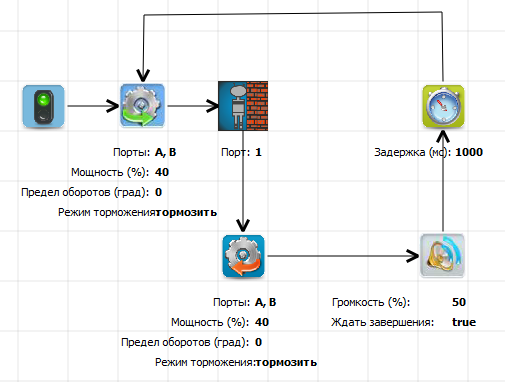
\includegraphics[width=0.7\textwidth]{programExample.png}
    \caption{Пример программы QReal:Robots}
    \label{programExample}
  \end{center}
\end{figure}

Все блоки языка делятся на несколько крупных смысловых групп, которые могут быть отдельно свёрнуты/развёрнуты в палитре. В языке присутствуют следующие блоки.
\begin{description}
	\item[Алгоритмы] --- блоки для управления вычислительным процессом и организации диаграмм.
  \begin{description}
    \item[Диаграмма поведения робота] --- позволяет создавать новые диаграммы. В каждый конкретный момент времени может быть выполнена или сгенерирована только одна диаграмма, но проект может содержать несколько диаграмм, между которыми можно переключаться.
    \item[Линия соединения] --- задаёт последовательность передачи управления между блоками.
    \item[Параллельные задачи] --- позволяет разделить поток управления на несколько параллельных потоков, которые будут исполняться независимо. Выглядит как блок, из которого выходит несколько соединительных линий, который при получении маркера управления создаёт несколько маркеров (по одному для каждой соединительной линии) и отправляет их каждому соединённому с ним блоку. После разделения задачи независимы.
    \item[Условие] --- оператор, проверяющий заданное логическое условие и, в зависимости от исхода проверки, передающий маркер управления на одну из двух исходящих соединительных линий. Поскольку в QReal, в отличие от LabView, у блока нет понятия "порт" в том смысле, что все исходящие линии равнозначны, одна из них должна быть помечена условием, по которому выполняется переход, а вторая должна быть не помечена. Непомеченной связи передаётся управление в том случае, если условие не выполнено.
    \item[Цикл] --- блок для задания аналога цикла "for" в текстовых языках. Блок должен иметь две исходящие связи, на одну из которых передаётся управление, пока цикл выполняется, когда цикл заканчивается, управление передаётся на вторую соединительную линию. Количество итераций задаётся как параметр блока.
  \end{description}
  \item[Действия] --- команды роботу.
  \begin{description}
    \item[Гудок] --- команда роботу издать звук.
    \item[Играть звук] --- команда роботу издать звук заданной частоты и громкости с заданной продолжительностью. Отличается от блока "Гудок" существенно большими возможностями в настройке.
    \item[Моторы вперёд] --- команда роботу включить моторы на заданных портах с заданной мощностью на заданное количество оборотов. Если число оборотов указано как 0, моторы будут работать неограниченно.
    \item[Моторы назад] --- команда роботу включить моторы в режиме движения назад с параметрами, аналогичными параметрам блока "Моторы вперёд".
    \item[Моторы стоп] --- команда роботу выключить моторы.
    \item[Функция] --- блок для записи произвольного математического выражения или кода на С.
  \end{description}
  \item[Инициализация] --- блоки, отвечающие за инициализацию робота и начало работы программы.
  \begin{description}
    \item[Блок инициализации] --- блок, обозначающий начало программы и позволяющий задать, на каком порту находится какой сенсор.
    \item[Конец] --- блок, обозначающий конец программы и отключение моторов и сенсоров робота.
    \item[Начало] --- блок, аналогично блоку инициализации обозначающий начало программы, но без параметров.
    \item[Сбросить показания энкодеров] --- блок, возвращающий значения счётчиков оборотов моторов в 0.
  \end{description}
  \item[Ожидания] --- блоки, передающие управление дальше только при наступлении какого-либо события.
  \begin{description}
    \item[Ждать интенсивность цвета] --- блок, продолжающий выполнение программы только в том случае, если значение, возвращаемое сенсором цвета на заданном порту, будет больше или меньше заданного значения.
    \item[Ждать свет] --- блок, продолжающий выполнение программы, если значение, возвращаемое сенсором освещённости на заданном порту, будет больше или меньше заданного значения.
    \item[Ждать сенсор касания] --- выполнение программы продолжается при срабатывании сенсора касания на заданном порту.
    \item[Ждать сонар] --- выполнение программы продолжается, если значение, которое вернул ультразвуковой сенсор расстояния, больше или меньше указанного значения.
    \item[Ждать цвет] --- выполнение программы будет продолжено, если сенсор цвета обнаружит заданный цвет.
    \item[Ждать энкодер] --- выполнение продолжится, если значение счётчика оборотов на указанном порту будет больше заданного.
    \item[Таймер] --- выполнение продолжится по истечении указанного промежутка времени (в миллисекундах).
  \end{description}
\end{description}

Язык позволяет везде, где можно указывать численный параметр, использовать математические выражения, включающие в себя арифметические действия, тригонометрические функции и переменные. Кроме того, имеется специальный блок "Функция", используемый для работы с математическими выражениями. В выражениях можно использовать текущие показания с помощью так называемых сенсорных переменных --- предопределённых переменных с именами Сенсор1, Сенсор2 и т.д., значения которых обновляются в соответствии с показаниями сенсоров. Пример программы, использующей математические выражения и сенсорные переменные, приведён на рисунке~\ref{movingAlongTheLine}. На рисунке изображена реализация алгоритма движения робота вдоль чёрной линии на полу по показаниям двух датчиков освещённости на основе пропорционально-дифференциального регулятора (подробнее см., например, в~\cite{filippov}).

\begin{figure} [ht]
  \begin{center}
    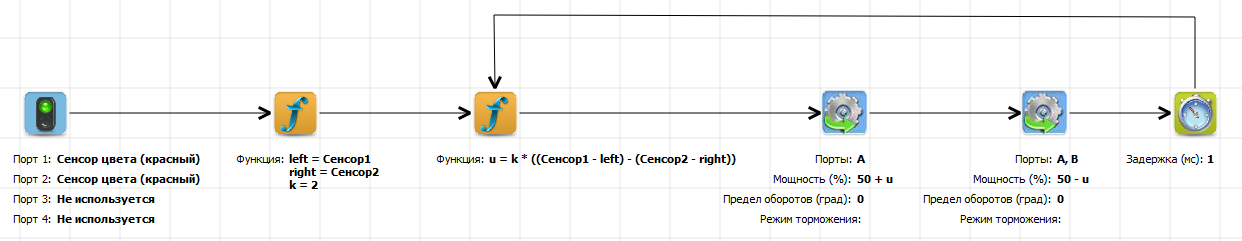
\includegraphics[width=\textwidth]{movingAlongTheLine.png}
    \caption{Движение вдоль линии}
    \label{movingAlongTheLine}
  \end{center}
\end{figure}

Язык QReal:Robots можно рассматривать как типичный пример предметно-ориентированного языка. Блоки языка отражают понятия из предметной области, а организация программы --- естественный процесс мышления при программировании робота, выстраивание последовательности команд. Важно, что программа на визуальном языке понятна пользователю, который даже впервые видит этот язык, но ориентируется в программировании роботов. Для этого используется такой приём, как использование для отображения блоков языка картинок, понятных людям, которые ориентируются в предметной области (описанный, например, в~\cite{theBook}). Например, на блоках, управляющих моторами, изображён мотор из конструктора Lego NXT, и все, кто хоть раз видел робот, по внешнему виду блока смогут понять его предназначение. Кроме того, оказалось важным, что передача управления между блоками изображается стрелками, это делает программу ещё более наглядной.

\section{Инструментальные средства QReal:Robots}
С помощью QReal оказалось легко создать визуальный язык, но инструментальные средства для него необходимо создавать вручную, поскольку такие задачи, как управление реальным роботом по Bluetooth, двухмерная модель робота и т.д. требуют ручного кодирования. Ниже следует краткое описание функциональности, реализованной вручную.

Инструментальная поддержка программирования роботов в QReal:Robots состоит из двух частей: интерпретатора диаграмм и генератора кода на C для загрузки на робот. Интерпретатор создавался с учётом следующих требований.
\begin{itemize}
  \item Возможность быстро задавать поведение для новых блоков визуального языка.
  \item Интерпретация диаграмм передачей роботу команд по Bluetooth или USB, в зависимости от выбора пользователя.
  \item Наличие двухмерной модели робота, которая могла бы интерпретировать диаграмму вместо реального робота. Двухмерная модель робота должна взаимодействовать с симулируемым окружением --- должно быть можно рисовать стены, линии и цветные области на полу.
  \item Архитектура должна позволять быстро поддержать новые виды оборудования, например, нестандартные сенсоры.
\end{itemize}

Архитектура интерпретатора приведена на рисунке~\ref{interpreterArchitecture}.

\begin{figure} [ht]
  \begin{center}
    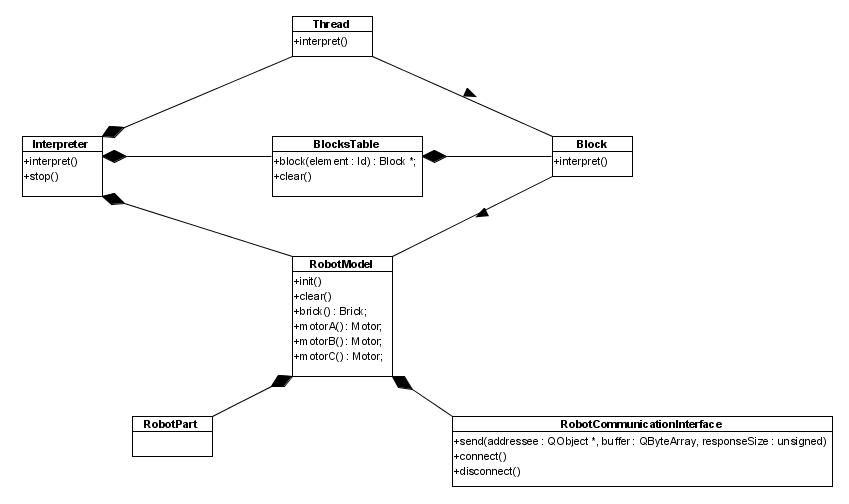
\includegraphics[width=0.7\textwidth]{interpreterArchitecture.jpg}
    \caption{Архитектура интерпретатора}
    \label{interpreterArchitecture}
  \end{center}
\end{figure}

Пользователь начинает интерпретацию диаграммы с помощью класса Interpreter, который хранит в себе контекст вычислений и контролирует потоки запущенной программы. Первое, что он делает --- обходит переданную на интерпретацию диаграмму, создавая для каждого блока объект, обеспечивающий его выполнение. При этом заполняется таблица блоков BlocksTable, ставящая в соответствие каждому идентификатору элемента на диаграмме такой объект, чтобы в дальнейшем иметь возможность быстро найти объект-исполнитель для передачи управления. После этого создаётся основной поток программы, содержащий в себе маркер исполнения. Маркер устанавливается на блок начала или инициализации, после чего проводится инициализация логической модели робота (класс RobotModel, в зависимости от настроек может реализовывать как управление реальным роботом, так и управление двухмерной моделью, для этого используется паттерн "стратегия"). После того, как инициализация закончена (для этого может потребоваться дождаться ответа от робота об инициализации оборудования), запускается метод interpret() блока, на котором находится маркер выполнения. Блок выполняется (для этого, опять-таки, может потребоваться асинхронная посылка команд на робот и ожидание ответа), после чего сообщает своему потоку, на какой следующий блок передать маркер управления. Так продолжается до тех пор, пока маркер управления потока не доходит до блока "Конец", после чего поток завершается.

Взаимодействие с реальным роботом осуществляется через реализации интерфейса RobotCommunicationInterface, который предоставляет возможность послать заданный пакет байтов на робот. Mindstorms NXT позволяет управлять собой командами по Bluetooth и по USB, поэтому в QReal:Robots имеется две реализации RobotCommunicationInterface. Управление по Bluetooth осуществляется через виртуальный COM-порт Bluetooth-соединения, обеспечиваемый средствами операционной системы, а управление по USB требует наличия установленного драйвера робота, и команды посылаются через драйвер. Каждый блок диаграммы реализован в терминах логической модели робота, логическая модель в случае работы с реальным роботом формирует управляющую команду и посылает её через RobotCommunicationInterface на робот. В случае с двухмерной моделью логическая модель вызывает методы классов, реализующих двухмерную модель, которые отрабатывают команды и формируют значения сенсоров.

Двухмерная модель моделирует робот с жёстко заданным расположением моторов, однако же позволяет настраивать расположение сенсоров. Поддерживаются сенсоры касания, расстояния, цвета. Двухмерная модель позволяет рисовать стены, линии и цветные области на полу. Внешний вид окна двухмерной модели представлен на рисунке~\ref{2dModel}.

\begin{figure} [ht]
  \begin{center}
    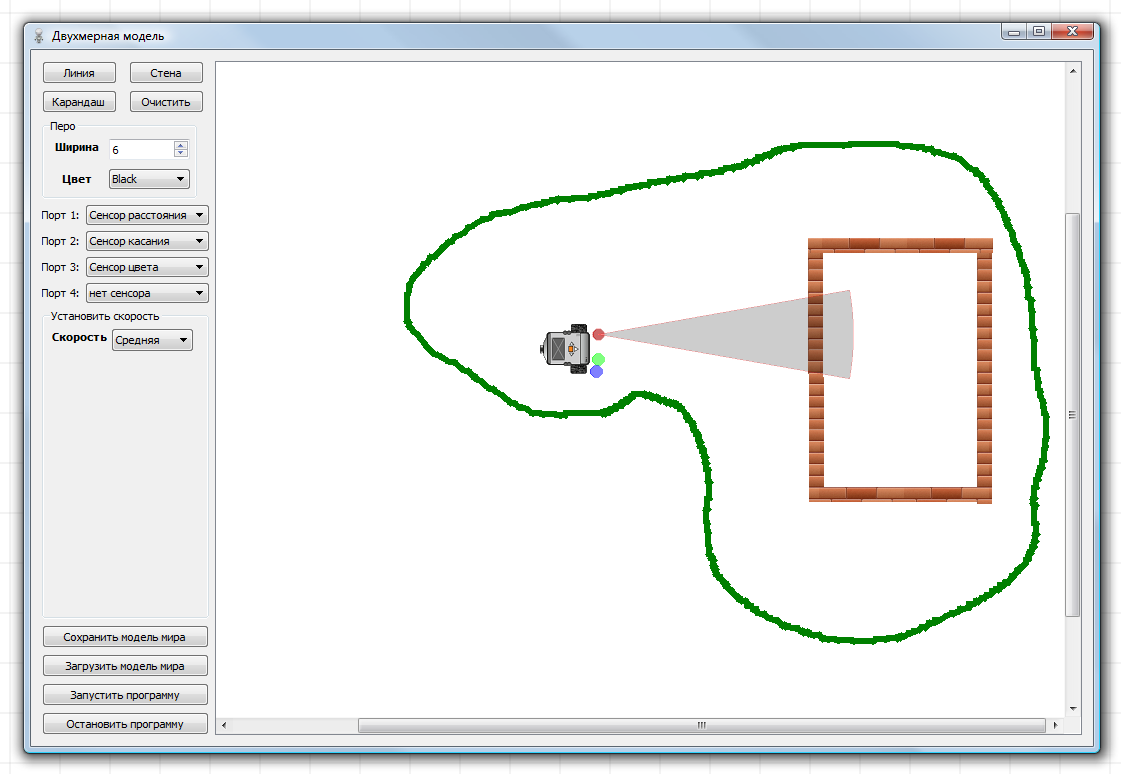
\includegraphics[width=0.7\textwidth]{2dModel.png}
    \caption{Окно двухмерной модели}
    \label{2dModel}
  \end{center}
\end{figure}

Генератор кода на C в QReal:Robots реализован в виде отдельного компонента, который может подключаться к основной программе независимо от интерпретатора. В качестве среды времени выполнения генератор использует операционную систему nxtOSEK~\cite{nxtOsek}, одну из самых быстрых доступных на данный момент операционных систем для роботов Lego. Генератор порождает .c-файл с кодом решения задачи и .oil-файл с настройками параметров выполнения кода. Далее автоматически запускается кросскомпилятор из состава nxtOSEK, собирающий эти файлы вместе с заголовочными файлами операционной системы, после чего получившийся бинарный образ загружается на робот по USB посредством утилиты, распространяемой с драйвером робота. Для пользователя этот процесс прозрачен, достаточно подключить робот, нажать кнопку "Загрузить программу на робот", после чего сгенерированный по диаграмме код программы покажется в окне встроенного в QReal текстового редактора, и одновременно начнётся процесс компиляции и загрузки программы.

Технически генератор реализован по шаблонной схеме, довольно типичной для генераторов кода по диаграммам в DSM-подходе~\cite{theBook}. Имеется шаблон порождаемого исходного кода, представляющий из себя почти готовую программу со специально размеченными местами, куда надо вставить код, сгенерированный по диаграмме. При генерации кода могут использоваться вспомогательные шаблоны --- как правило, небольшие фрагменты программы, параметризуемые информацией из диаграммы. Небольшой пример шаблона приведён ниже:
\begin{verbatim}
void ecrobot_device_initialize(void)
{
@@INITHOOKS@@
}
\end{verbatim}
Здесь на место \verb|@@INITHOOKS@@| вставляется код, сгенерированный по блоку инициализации диаграммы, а всё остальное попадает в выходной файл без изменений. По каждому блоку генерируется свой небольшой фрагмент программы, при этом некоторую сложность представляют структурные операторы, например, циклы или условные переходы. Проблема в том, что диаграмма может быть нарисована неструктурно, синтаксис визуального языка не запрещает делать, например, условный переход внутрь тела цикла, или условный переход наружу из тела другого оператора if. С точки зрения визуального языка, такие ситуации абсолютно корректны, но в тектовое представление переводятся только с использованием операторов goto (или техник goto elimination, известных в реинжиниринге). Однако, поскольку сгенерированный код предполагается использовать в иллюстративных целях, использовать оператор goto было бы крайне нежелательно. Генератор применяет набор эвристик, позволяющих найти на диаграмме фрагменты, соответствующие структурным операторам if, циклам while и do/while. В случае, если генератор не может породить структурный код по данной диаграмме, выдаётся ошибка и код не порождается вообще. Интерпретация такой диаграммы, тем не менее, вполне возможна.

\section{Опыт применения QReal}
\subsection{Создание редактора языка}
Визуальный язык для QReal:Robots создавался с помощью метаредактора QReal. Полная метамодель одной из версий языка представлена на рисунке~\ref{robotsMetamodel}. Как видно, она целиком помещается на одном экране. Все элементы также имеют свойства (в том числе, внешний вид), которые на рисунке не показаны.

\begin{figure} [ht]
  \begin{center}
    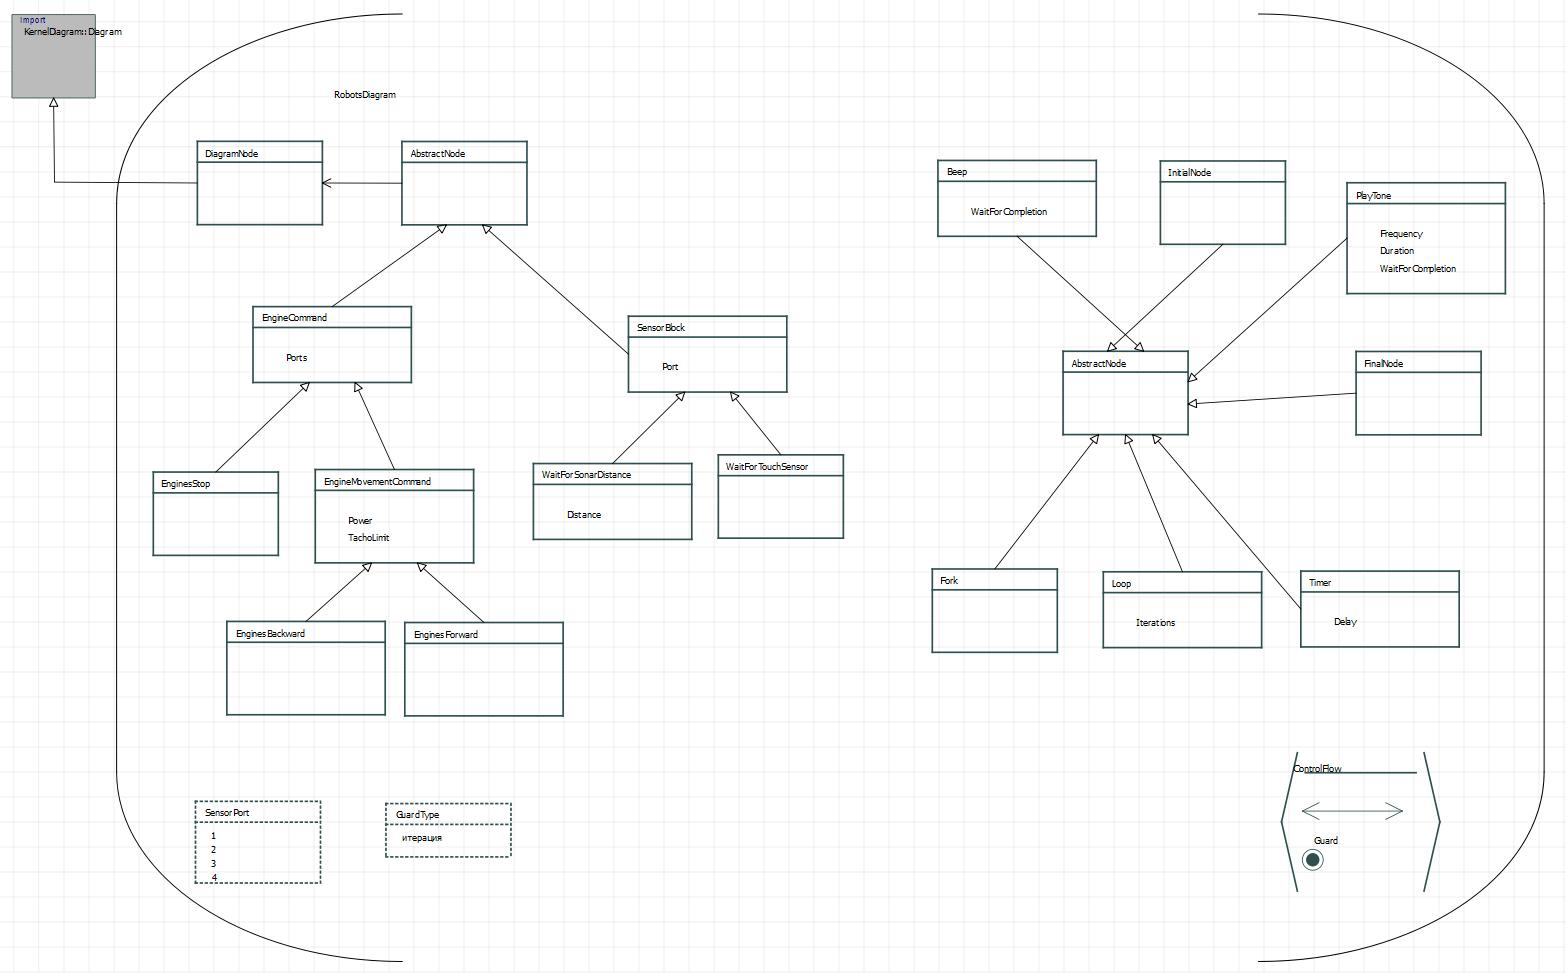
\includegraphics[width=\textwidth]{robotsMetamodel.jpg}
    \caption{Метамодель языка QReal:Robots}
    \label{robotsMetamodel}
  \end{center}
\end{figure}

Корневой сущностью метамодели является диаграмма, в неё помещаются все элементы языка. Диаграмма --- вкладка в палитре блоков, в неё добавляются все блоки языка, все виды связей, все перечислимые типы, используемые в свойствах элементов, и т.д. Одна метамодель может содержать несколько диаграмм, тогда плагин-редактор, сгенерированный из этой метамодели, при загрузке будет добавлять несколько вкладок в палитру. Внутри диаграммы находятся узлы --- элементы визуального языка. Узлы могут быть связаны отношением наследования и отношением "содержит". Отношение "содержит" указывает, что один узел может содержать другой в себе, то есть являться контейнером для этого узла. В языке программирования роботов узел "диаграмма" связан отношением "содержит" с узлом AbstractNode, узлом-предком всех узлов языка, таким образом, диаграмма может содержать все элементы. Больше, в силу простоты языка, отношение "содержит" в метамодели не используется. Отношение наследования в метамодели можно понимать как обычное наследование в объектно-ориентированных языках программирования --- узел-потомок может использоваться везде, где может использоваться узел-предок, и наследует все его свойства. В метамодели языка программирования роботов наследование оказалось довольно удобным инструментом: узел "диаграмма" наследуется от импортированного из другой метамодели узла "диаграмма", все другие узлы наследуются от узла AbstractNode. Заметим, что AbstractNode на одной диаграмме представлен дважды --- это два образа одного и того же логического элемента модели. Это иллюстрирует важную особенность QReal --- разделение логической и графической модели системы. Генераторы и другие инструменты работают с логической моделью, пользователь может редактировать графическую модель, которая связана с логической, но может отличаться. Например, один и тот же элемент может отображаться на нескольких разных диаграммах, или даже в нескольких местах одной диаграммы, это позволяет рисовать диаграммы, представляющие одни и те же сущности с разных точек зрения. В метамодели языка программирования роботов второй образ AbstractNode использован для удобства отображения, чтобы уменьшить количество пересекающихся линий.

От AbstractNode наследуются абстрактные узлы команд моторов (EngineCommand) и сенсоров (SensorBlock). Абстрактные узлы не отображаются в палитре, поскольку для них не задаётся графическое представление, однако, туда вынесены общие свойства узлов-наследников. От EngineCommand наследуется один конкретный блок (EngineStop, остановка мотора) и один абстрактный (EngineMovementCommand, команда движения). От EngineMovementCommand наследуются два конкретных блока "моторы вперёд" и "моторы назад", которые своих свойств не имеют, и их семантика определяется помимо свойств узла-родителя их типом. 

Свойства внутри узла имеют имя, тип и значение по умолчанию. Тип свойства определяет, какие допустимые значения может принимать свойство, и как будет осуществляться редактирование значений в редакторе свойств. Например, для строкового свойства в редакторе свойств будет показано поле ввода, для булевого свойства --- "галочка", для перечислимого типа --- выпадающий список с возможными значениями. Перечислимые типы определяются в метамодели языка, в метамодели языка роботов, например, определён тип-перечисление SensorPort, принимающий значения 1, 2, 3, 4, и используемый как тип свойств, определяющих порты сенсоров. Кроме типов-перечислений, в метамодели задаются виды связей, для которых указывается то, как их следует отрисовывать (заполненные или пустые стрелки, ромбы и т.д. на каждом из концов связи, пунктирная или сплошная линия, и т.д.), свойства, то, к каким узлам связь можно присоединять.

После того, как метамодель нарисована, с помощью редактора форм фигур задаются изображения для элементов. После этого можно сгенерировать редактор. Вообще, получить из метамодели редактор визуального языка в QReal можно тремя способами, представленными на рисунке~\ref{editorGeneration}.

\begin{figure} [ht]
  \begin{center}
    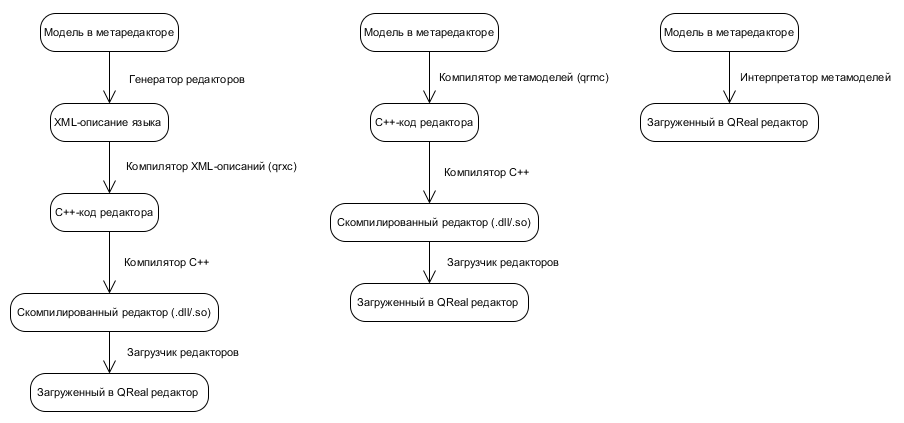
\includegraphics[width=0.7\textwidth]{editorGeneration.png}
    \caption{Способы генерации редактора в QReal}
    \label{editorGeneration}
  \end{center}
\end{figure}

Первый способ используется наиболее часто и предполагает использование промежуточного xml-формата представления метамодели. Пока метаредактора в QReal не существовало, все метамодели задавались вручную в xml-файлах, по которым затем порождался код на C++, компилировался, и подключался к основной части системы как динамически загружаемая библиотека. С появлением метаредактора в эту схему добавился генератор, порождающий по метамодели, хранящейся в репозитории, xml-файл с описанием метамодели. Второй способ был реализован позже и предполагает генерацию кода на C++ непосредственно по метамодели, без порождения промежуточного представления. Такой способ проще, но менее устойчив к изменениям в метаязыке --- если удалить какой-либо элемент метаязыка или даже какое-либо его свойство, старые метамодели, содержащие удалённый элемент, окажется невозможно загрузить и отредактировать. В xml-файлы в таких ситуациях изменения несложно внести вручную, редактировать вручную файлы с сохранёнными метамоделями гораздо сложнее. Поэтому второй способ не используется в процессе сборки QReal, а существует как альтернативный, до тех пор, пока не будет создано надёжного средства поддержки эволюции языков. На данный момент в процессе сборки QReal все плагины-редакторы (включая метаредактор) собираются из xml-файлов с метамоделями. Третий способ предполагает не генерацию по метамодели кода, реализующего редактор, а непосредственную интерпретацию метамодели в интерпретаторе, эмулирующем функциональность плагина-редактора. Такой способ технически наиболее удобен, поскольку для создания редактора не будет требоваться компилятор C++, и не требуется порождения никаких промежуточных представлений, однако же, интерпретируемый редактор работает медленнее сгенерированного. Интерпретатор может обладать рядом возможностей, недоступных сгенерированным редакторам, таким как модификация визуального языка "на лету", но на данный момент эти возможности в QReal не реализованы.

\subsection{Выводы}
Среду QReal:Robots вряд ли удалось бы разработать в столь короткие сроки вручную. Использование metaCASE-системы QReal позволило существенно упростить создание визуального языка и редактора диаграмм для него. Прототип языка был готов за несколько часов, так что уже после недели разработки первый функциональный прототип среды программирования, включающий в себя редактор диаграмм и интерпретатор, управляющий роботом по Bluetooth, был представлен специалистам по кибернетике. При создании языка наиболее затратным по времени оказался поиск подходящих иконок для блоков диаграммы. Создание метамодели языка с помощью метаредактора оказалось довольно быстрым, первая версия языка содержала порядка десятка блоков, находящихся друг с другом в несложных отношениях, и с тех пор язык лишь незначительно вырос, вся его метамодель в графическом виде помещается на один экран. Поскольку редактор диаграмм языка по метамодели генерируется автоматически, была возможность не только сэкономить время на разработке редактора, но и экспериментировать с языком, меняя блоки, их свойства и внешний вид. Кроме того, простота визуального представления синтаксиса языка дала возможность легко расширять и изменять его в дальнейшем, причём не только исходным авторам языка. Впоследствии разработка QReal:Robots была во многом передана студентам, которые без особых сложностей редактировали и расширяли язык по мере необходимости. Рассматривалась даже возможность позволить самим пользователям менять язык, например, дать возможность учителям информатики настраивать язык под конкретное занятие, но такая возможность до сих пор не была реализована в силу недоработанности средств метамоделирования в QReal.

Если синтаксис языка оказался хорошо формализуемым и процесс построения редактора языка по описанию синтаксиса удалось автоматизировать, то с семантикой ситуация оказалась хуже. Система QReal на момент разработки QReal:Robots не имела никаких средств описания семантики языка, так что вся инструментальная поддержка, включая интерпретатор диаграмм и генератор кода для заливки на робот, реализовывалась вручную, программированием на C++. Эта задача трудоёмка и сама по себе --- требовалось изучить систему прямых команд робота для управления им с компьютера, изучить API операционной системы робота для генерации кода для неё, наладить работу с Bluetooth, USB, кросскомпиляцию, прошивку робота, загрузку программы на робот и прочие проблемы, не автоматизируемые в принципе. Однако же, некоторый код получился довольно шаблонным --- каждому блоку соответствовал некоторый класс на С++, реализовывавший его функциональность при интерпретации, и по крайней мере шаблоны для таких классов можно было бы генерировать автоматически по описанию языка. Интерпретатор в целом также мало связан конкретно с языком программирования роботов, так что, возможно, часть его можно было бы генерировать по описанию семантики языка, представленной в каком-то виде, а часть вынести в библиотеку и использовать в сгенерированном коде. Предполагается, что использование интерпретируемых языков программирования для описания части поведения интерпретатора позволило бы ускорить разработку, но эта идея ещё не была проверена.

Генератор кода представляется наиболее интересной целью для автоматизации, поскольку содержит много похожего от блока к блоку кода. Как и интерпретатор, генератор содержит неспецифичные для языка программирования роботов части, которые были бы применимы для всех визуальных языков с семантикой, похожей на семантику диаграмм активностей UML или блок-схем. Над автоматизацией создания генератора в QReal в данный момент ведётся работа, был создан язык описания правил генерации, берущий на себя многие типичные задачи, такие как обход графа модели и вывод текста. Тем не менее, такой язык не позволяет выполнять сложные алгоритмические действия, например, goto elimination или поиск переменных в математических выражениях для дальнейшей автоматической генерации блока объявления переменных.

Таким образом, результатом эксперимента по разработке системы визуального программирования с помощью metaCASE-системы стало то, что с помощью такого подхода можно создать систему, которая была бы не хуже разработанных вручную, и при этом время на разработку визуального редактора с помощью метамоделирования можно сократить в несколько десятков раз по сравнению с разработкой редактора вручную. Однако выигрыш при разработке и доведении до внедрения системы в целом оказался не таким значительным, как при разработке только редактора, потому как многие задачи принципиально неавтоматизируемы. В процессе эксперимента были выявлены типичные при разработке подобного рода систем задачи, которые можно в некоторой степени автоматизировать в metaCASE-системе, но их автоматизация требует дополнительных исследований. Большая часть таких задач требует изучения способов задания семантики визуальных языков. Однако даже сейчас DSM-подход показал себя полезным на практике, и представляется, что дальнейшие исследования в этом направлении смогут помочь эффективно создавать специализированные языки и среды программирования даже для гораздо более узких предметных областей и задач.

\section*{Заключение}
В результате применения описанного в статье подхода удалось разработать полноценную среду программирования роботов, которую оказалось возможным предложить школьникам и учителям в качестве замены используемых ныне в школах средств. QReal:Robots была представлена на "Открытых состязаниях Санкт-Петербурга по робототехнике" и на робототехническом фестивале "Робофест 2012" в Москве. В качестве доказательства применимости среды QReal:Robots к реальным задачам, решаемым школьниками, команда студентов приняла участие в соревнованиях в движении робота по линии с программой, реализованной целиком на QReal:Robots. Задача движения по линии состоит в том, что руководствуясь показанием датчиков освещённости робот должен проехать по нарисованной на полу кривой замкнутой чёрной линии за возможно меньшее время. Несмотря на то, что для студентов участие в соревнованиях стало практически первым опытом решения задач робототехники, им удалось показать довольно неплохие результаты, заняв места в середине таблицы, несмотря на то, что довольно многие участники использовали специально созданные для этой задачи роботы. QReal:Robots представлялся также в виде стендовых докладов, где вызвал большую заинтересованность у потенциальных пользователей. Было проведено анкетирование удобства пользовательского интерфейса, которое показало, что продукт достаточно хорош, чтобы вызывать у пользователей симпатию и желание им пользоваться.

Эксперимент показал применимость DSM-подхода для разработки средства визуального программирования, которое может распространяться как отчуждаемый продукт и рассчитано на аудиторию, не владеющую программированием. При этом использование средств автоматизации создания редакторов сэкономило много времени и усилий. Также в процессе эксперимента было выявлено несколько направлений, кажущихся перспективными для дальнейшей автоматизации.

\begin{thebibliography}{9001}

  \bibitem{robots} \emph{Брыксин Т.А., Литвинов Ю.В.} Среда визуального программирования роботов QReal:Robots // Материалы международной конференции ``Информационные технологии в образовании и науке''. Самара. 2011. С. 332--334.
  
  \bibitem{legoNxt} LEGO Mindstorms homepage, URL: http://mindstorms.lego.com/en-us/Default.aspx (дата обращения: 14.07.2012)
  
  \bibitem{logo} MyRobot, Язык программирования Лого, URL: http://myrobot.ru/logo/aboutlogo.php (дата обращения: 22.07.2012)
  
  \bibitem{logoTurtle} cyberneticzoo.com, 1969 – The Logo Turtle – Seymour Papert et al, URL: http://cyberneticzoo.com/?p=1711 (дата обращения: 20.07.2012)
  
  \bibitem{robolab} \emph{Portsmore, Merredith} ROBOLAB: Intuitive Robotic Programming Software to Support Life Long Learning, APPLE Learning Technology Review, Spring/Summer 1999
  
  \bibitem{robolabHome} Robolab home page, URL: http://www.ceeo.tufts.edu/robolabatceeo/ (дата обращения: 14.07.2012)
  
  \bibitem{mrds} Microsoft Robotics Developer Studio homepage, URL: http://www.microsoft.com/robotics/ (дата обращения: 22.07.2012)
  
  \bibitem{mrdsAtMySpace} \emph{Michael S. Scherotter}, CCR at MySpace, URL: http://channel9.msdn.com/Shows/Communicating/CCR-at-MySpace (дата обращения: 01.07.2012)
  
  \bibitem{videoDsl} \emph{Кознов Д.В., Перегудов А.Ф., Бугайченко Д.Ю. и др.} Визуальная среда проектирования систем телевизионного вещания // Системное программирование. 2006. Т. 2. № 1. С. 142-168.
  
  \bibitem{dsmPlatforms} \emph{Павлинов А.А., Кознов Д.В., Перегудов А.Ф. и др.} О средствах разработки проблемно-ориентированных визуальных языков // Системное программирование. 2006. Т. 2. № 1. С. 116-141.
  
  \bibitem{robik} \emph{Звенигородский Г.А.} Описание языка Робик, URL: http://ershov.iis.nsk.su/archive/eaindex.asp?lang=1\&did=7639 (дата обращения: 20.07.2012)
  
  \bibitem{real1} \emph{Иванов А., Кознов Д., Лебедев А. и др.} Объектно-ориентированное расширение технологии RTST. // Записки семинара кафедры системного программирования <<CASE-средства RTST++>>. Вып. 1. - CПб, Изд-во С.-Пб ун-та, 1998. С. 17-36.
  
  \bibitem{real2} \emph{Терехов А.Н., Романовский К.Ю., Кознов Д.В. и др.} REAL: методология и CASE-средство для разработки систем реального времени и информационных cистем, Программирование, 1999, № 5. C. 44-52.

  \bibitem{theBook} \emph{Kelly, S., Tolvanen, J.} Domain-Specific Modeling: Enabling Full Code Generation // Wiley-IEEE Computer Society Press. 2008. 448 pp.

  \bibitem{qReal} \emph{Терехов А.Н., Брыксин Т.А., Литвинов Ю.В. и др.} Архитектура среды визуального моделирования QReal. // Системное программирование. Вып. 4. СПб.: Изд-во СПбГУ. 2009, С. 171-196
  
  \bibitem{mythicalManMonth} \emph{Брукс Ф.} Мифический человеко-месяц, или Как создаются программные системы, Символ-Плюс, 2010г. 304 С.
  
  \bibitem{filippov} \emph{Филиппов С.А.} Робототехника для детей и родителей, Наука, 2011г. 264 С.
  
  \bibitem{kelly} \emph{Kelly, S., Tolvanen, J.-P.}, Visual domain-specific modeling: benefits and experiences of using metaCASE tools, in: Bezivin, J., Ernst, J. (Eds.), Proceedings of International workshop on Model Engineering, ECOOP 2000
  
  \bibitem{kieburtz} \emph{Kieburtz, R., et al.} A software engineering experiment in software component generation, Proceedings of 18th International Conference on Software Engineering, Berlin, IEEE Computer Society Press, March, 1996

  \bibitem{weiss} \emph{Weiss, D., Lai, C. T. R.}, Software Product-line Engineering, Addison Wesley Longman, 1999.
  
  \bibitem{gmp} Graphical Modeling Project homepage, URL: http://www.eclipse.org/modeling/gmp/ (дата обращения: 05.08.2012)
  
  \bibitem{vsvmsdk} Visual Studio Visualization and Modeling SDK (was DSL SDK), URL: http://archive.msdn.microsoft.com/vsvmsdk (дата обращения: 05.08.2012)
  
  \bibitem{metaEditPlus} MetaEdit+ homepage, URL: http://www.metacase.com/ (дата обращения: 05.08.2012)
  
  \bibitem{visio} Microsoft Visio homepage, URL: http://office.microsoft.com/ru-ru/visio/ (дата обращения: 05.08.2012)
  
  \bibitem{xmi} MOF/XMI specification, URL: http://www.omg.org/spec/XMI/2.4.1/ (дата обращения: 05.08.2012)
  
  \bibitem{qRealGithub} Домашнаяя страница проекта QReal на GitHub, URL: https://github.com/qreal/qreal (дата обращения: 05.08.2012)
  
  \bibitem{nxtOsek} nxtOSEK homepage, URL: http://lejos-osek.sourceforge.net/ (дата обращения: 12.08.2012)
  
  \bibitem{student1} \emph{Терехов А.Н., Кияев В.И., Комаров С.Н.} Принципы информатизации системы управления в Санкт-Петербургском Государственном Университете // Вестник Санкт-Петербургского университета, Серия 8: Менеджмент, 2004, № 2, С. 151-200.
  
  \bibitem{student2} \emph{Комаров С.Н., Терехов А.Н., Граничина О.А.} Интегрированно-распределённая автоматизированная информационная система для крупного научно-образовательного учреждения // Вестник Санкт-Петербургского университета. Серия 10: Прикладная математика. Информатика. Процессы управления. 2008. № 1. С. 87-94. 

\end{thebibliography}

\end{document}
